%%%%%%%%%%%%%%%%%%%%%%%%%%%%%%%%%%%%%%%%%%%%%%%%%%%%%%%%%%%%%%%%%%%%%%
% Lớp 11 | Đạo hàm | Các quy tắc đạo hàm
% Dạng 1D7?2-8: Toán thực tế áp dụng quy tắc đạo hàm
% Số câu: 52  (sinh tự động bởi tach_cau.py; từ nay thầy sửa trực tiếp file này)
%%%%%%%%%%%%%%%%%%%%%%%%%%%%%%%%%%%%%%%%%%%%%%%%%%%%%%%%%%%%%%%%%%%%%%

%%%%%%%%%%%%%%%% TRẮC NGHIỆM 4 PHƯƠNG ÁN %%%%%%%%%%%%%%%%

% nguồn: Ok_TracNghiemLop11_Lan1
\begin{ex}%[1D7N2-8]%[ma:517601a0]
	Một vật chuyển động có phương trình $S=t^4-3t^3-3t^2+2t+1$ (m) $t$ là thời gian tính bằng giây. Gia tốc của  vật tại thời điểm $t=3$ s là
	 \choice
		{\True  $48$ m/s$^2$}
		{$28$  m/s$^2$}
		{$18$ m/s$^2$} 
		{$54$  m/s$^2$}
	\loigiai{ 
		 $S=f\left(t\right)=t^4-3t^3-3t^2+2t+1$.\\
		$\Rightarrow  f'\left(t\right)=4t^3-9t^2-6t+2$.\\
		$\Rightarrow a\left(t\right)=f''\left(t\right)=12t^2-18t-6$.\\ 
	Gia tốc của vật tại thời điểm $t=3$ là $a\left(3\right)=12\cdot 3^2-18\cdot 3-6=48$ m/s$^2$.} 
\end{ex}

% nguồn: Ok_TracNghiemLop11_Lan1
\begin{ex}%[1D7N2-8]%[ma:f5ab6bf9]
	Cho chuyển động được xác định bởi phương trình $S(t)=t^{3}-3t^{2}+t+11$, trong đó $t$ được tính bằng giây và $S$ được tính bằng mét. Vận tốc của chuyển động khi $t=2$  giây là
	\choice 
		{$9$ m/s} 
		 {$6$ m/s}
		 {$-3$ m/s}
		{\True $1$  m/s}
	 \loigiai{
		Ta có $S'(t)=3t^{2}-6t+1\Rightarrow  v(2)=S'(2)=1$.
	 }
\end{ex}

% nguồn: Ok_TracNghiemLop11_Lan1
\begin{ex}%[1D7H2-8]%[ma:a27327f4]
	Xét chuyển động có phương trình $s(t)=A\sin \left(\omega  t+\varphi \right)$, với $A,\omega,\varphi $ là những hằng số. Tìm gia tốc $\gamma(t)$ tại thời điểm $t$ của chuyển động.
	\choice 
		 {$\gamma (t)=A\omega \cos \left(\omega t+\varphi \right)$}
		{$\gamma (t)=A\omega^2\sin  \left(\omega t+\varphi \right)$}
		{\True $\gamma (t)=-A\omega^2\sin \left(\omega t+\varphi \right)$} 
		{$\gamma (t)=-A\omega  \cos \left(\omega t+\varphi \right)$}
	\loigiai{ 
		$s'(t)=A{\left(\omega t+\varphi \right)}'\cos \left(\omega t+\varphi \right)=A\omega \cos \left(\omega t+\varphi \right)$. \\ 
	Gia  tốc $\gamma (t)=s''(t)=-A\omega {\left(\omega t+\varphi \right)}'\sin \left(\omega t+\varphi \right)=-A\omega^2\sin \left(\omega t+\varphi \right)$.}
\end{ex}

% nguồn: Ok_TracNghiemLop11_Lan1
\begin{ex}%[1D7H2-8]%[5-CTST]%[ma:d44bb383]
	Một vật chuyển động theo quy luật $s = -\dfrac{1}{2}t^3 + 9t^2$ với $t$ (giây) là khoảng thời gian tính từ lúc bắt đầu chuyển động và $s$ (mét) là quãng đường vật đi được trong khoảng thời gian đó. Hỏi trong khoảng thời gian $10$ giây, kể từ lúc vật bắt đầu  chuyển động, vận tốc lớn nhất của vật đạt được bằng bao nhiêu?
	 \choice
		{$216~\left(m/s  \right)$}
		{$30~\left(m/s \right)$} 
		{$400~\left(m/s \right)$} 
		{\True $54~\left(m/s  \right)$}
	 \loigiai{
		Vận tốc tại thời  điểm $t$ là $v(t) = s'(t) = -\dfrac{3}{2}t^2 + 18t$ với $t \in \left[0; 10 \right]$.\\
		Ta có  $v'(t) = -3t + 18 = 0 \Leftrightarrow t = 6$.\\
		Suy ra $v(0) = 0$; $v(10) = 30$; $v(6) = 54$.\\ 
		Vậy  vận tốc lớn nhất của vật đạt được bằng $54~\left(m/s \right)$.
	 }
\end{ex}

% nguồn: Ok_TracNghiemLop11_Lan1
\begin{ex}%[1D7H2-8]%[ma:52b75fa8]
	Cho chuyển động được xác định bởi phương trình $s=2t^3+6t^2-t$, trong đó $t$ được tính bằng giây và $s$ được tính bằng mét. Vận tốc tức thời của chuyển động tại thời điểm $t=3$  s là
	 \choice
		{\True $89$ m/s} 
		{$105$  m/s}
		{$48$  m/s}
		{$20$ m/s} 
	 \loigiai{
		Ta có  $v(t)=S'(t)=6t^2+12t-1$.\\
	Vận tốc tức  thời của chuyển động khi $t=3$ s là $v(3)=6\cdot 3^2+12\cdot 3-1=89$ m/s.}
\end{ex}

% nguồn: Ok_TracNghiemLop11_Lan1
\begin{ex}%[1D7H2-8]%[ma:b21706a8]
	Một vật  chuyển động theo quy luật $s(t)=-\dfrac{1}{2}t^3+12t^2$, $t$ (giây) là khoảng thời gian tính từ lúc vật bắt đầu chuyển động, $s$ (mét) là quãng đường vật chuyển động trong $t$ giây. Vận tốc tức thời của vật tại thời điểm $t=10$ (giây) là
	\choice 
		 {$80$ (m/s)}
		{\True  $90$ (m/s)}
		{$100$ (m/s)} 
		{$70$  (m/s)}
	\loigiai{ 
		Vận tốc tức thời  của vật tại thời điểm $t$ là $v\left(t\right)=s'(t)=-\dfrac{3}{2}t^2+24t$.\\
	Vận tốc tức thời của vật tại  thời điểm $t=10$ (giây) là $v\left(10\right)=-\dfrac{3}{2}\cdot10^2+24\cdot10=90$ (m/s).}
\end{ex}

% nguồn: Ok_TracNghiemLop11_Lan1
\begin{ex}%[1D7V2-8]%[ma:aec61074]
	Một chất  điểm chuyển động thẳng được xác định bởi phương trình $s=t^3-3t^2+5t+2$, trong đó $t$ tính bằng giây và $s$ tính bằng mét. Gia tốc của chuyển động khi $t=3$ là:
	\choice 
		{\True $12$  m/s$^2$}
		{$17$  m/s$^2$}
		 {$24$ m/s$^2$}
		{$14$ m/s$^2$} 
	 \loigiai{
		Ta có vận tốc  của chuyển động $v(t)=s'(t)=3t^2-6t+5$.\\
		Gia tốc của chuyển  động $a(t)=v'(t)=6t-6$.\\
		Khi $t=3$, ta được $a(3)=12$  m/s$^2$.
	} 
\end{ex}

% nguồn: Ok_TracNghiemLop11_Lan1
\begin{ex}%[1D7V2-8]%[ma:4647b51c]
	Một chất điểm chuyển động có vận tốc tức thời $v(t)$ phụ thuộc vào thời  gian $t$ theo hàm số $v(t)=-t^4+8t^2+500$. Trong khoảng thời gian $t=0$ đến $t=5$ chất điểm đạt vận tốc lớn nhất tại thời điểm nào?
	 \choice
		 {$t=1$}
		 {$t=4$}
		{\True $t=2$} 
		 {$t=0$}
	\loigiai{ 
		Ta tính $v'(t)=-4t^3+16t=0\Leftrightarrow  \hoac{&{t=0} \\&{t=-2\text{ (loại)}} \\&{t=2.}}$\\
		Ta  có $v(0)=500$, $v(2)=516$, $v(5)=75$.\\
		Hàm số $v(t)$ liên tục trên $\left[0;5\right]$ nên  chất điểm đạt vận tốc lớn nhất tại thời điểm $t=2$.
	} 
\end{ex}


%%%%%%%%%%%%%%%% ĐÚNG/SAI %%%%%%%%%%%%%%%%

% nguồn: Ok_dungsai_lop11_Lan1
\begin{ex}%[1D7H2-8]%[ma:ed9e0b6d]
 Phương trình chuyển động của một hạt được cho bởi công thức $s(t)=10+\sqrt{2}\sin\left(\dfrac{\pi}{4}+4\pi t\right)$, trong đó  $s$ tính bằng centimet và $t$ được tính bằng giây. Xét tính đúng sai của các mệnh đề sau
  \choiceTF
  {Gia tốc của hạt tại  thời điểm $t=3$ giây là $-16\pi^2$ cm/s$^2$}
  {\True Vận tốc của hạt tại  thời điểm $t=3$ giây là $2\pi$ cm/s}
  {\True Vận tốc lớn nhất của hạt đạt được  là $4\pi\sqrt{2}$ cm/s}
  {Gia tốc nhỏ nhất của hạt đạt được là $-16\pi^2$  cm/s$^2$}
 \loigiai{ 
  Ta  có\\
   Vận tốc của hạt tại thời điểm $t$ là $v(t)=s'(t)=4\pi \sqrt{2}\cos\left(\dfrac{\pi}{4}+4\pi t\right)$.\\
  Gia tốc của hạt tại thời điểm $t$ là $a(t)=s''(t)=-16\pi ^2\sqrt{2}\sin\left(\dfrac{\pi}{4}+4\pi t\right)$. 
  \begin{itemchoice}
   \itemch Sai. Tại thời điểm $t=3$ giây thì gia  tốc của hạt là $$a=-16\pi^2\sqrt{2}\sin\left(\dfrac{\pi}{4}+12\pi \right)=-8\pi^2\text{ cm/s}^2.$$
   \itemch Đúng. Tại thời điểm $t=3$ giây thì vận  tốc của hạt là $$v=4\pi\sqrt{2}\cos\left(\dfrac{\pi}{4}+4\pi\cdot 3\right)=2\pi \text{ cm/s.}$$
   \itemch Đúng. Ta  có $-4\pi\sqrt{2}\leq 4\pi\sqrt{2}\cos\left(\dfrac{\pi}{4}+4\pi t\right)\leq 4\pi\sqrt{2}$ nên vận tốc lớn nhất của hạt đạt được là $4\pi\sqrt{2}$ cm/s.
   \itemch  Sai. Ta có $-16\pi^2\sqrt{2}\leq -16\pi^2\sqrt{2}\sin\left(\dfrac{\pi}{4}+4\pi t\right)\leq 16\pi^2\sqrt{2}$ nên gia tốc nhỏ nhất của hạt đạt được là $-16\pi^2\sqrt{2}$ cm/s$^2$.
  \end{itemchoice}
  }
\end{ex}

% nguồn: Ok_dungsai_lop11_Lan2
\begin{ex}%[1D7H2-8]%[ma:fbb287db]
	Một  chất điểm chuyển động thẳng được xác định bởi phương trình $s(t)=t^3-3t^2+5t+2$ trong đó $t$ tính bằng giây và $s$ tính bằng mét.
	 \choiceTF
		{\True Quãng  đường tại thời điểm $3$ giây là $17$\,m}
		{\True Vận tốc của chất điểm trong thời gian $4$ giây là  $29$\,m/s}
		{\True Tại thời điểm $t=1$\,s thì gia  tốc của chất điểm bằng $0$}
		{Trong khoảng thời gian từ $2$ giây đến  $5$ giây thì chất điểm chuyển động được $85$\,m}
	\loigiai{ 
		\begin{itemchoice}
			\itemch Quãng đường tại thời điểm $3$ giây thì  $s(3)=3^3-3\cdot 3^2+5\cdot 3+2=17$\,m.
			\itemch Vận tốc của chất điểm trong thời  gian 4 giây là $v(4)=s'(4)$, với $v(t)=s'(t)=3t^2-6t+5$.\\
			Suy  $v(4)=29$\,m.
			\itemch Ta có gia tốc  $a(t)=s''(t)=6t-6$, $\Rightarrow a(1)=0$
			\itemch Ta có $s(2)=8$\,m và $s(5)=77$\,m nên quãng đường chất điểm di chuyển từ $2$ giây đến $5$ giây là  \[s(5)-s(2)=77-8=69\,\mathrm{m}.\]
		\end{itemchoice}
	 }
\end{ex}

% nguồn: Ok_dungsai_lop11_Lan2
\begin{ex}%[1D7H2-8]%[ma:45a5032c]
	Một vật chuyển động trên đường thẳng được xác định bởi công thức $s(t)=-t^3+3t^2+9t+2$, trong đó $t > 0$ và tính bằng giây và $s$ là quãng đường chuyển động  được của vật trong $t$ giây tính bằng mét.
	\choiceTF 
		{\True Vận tốc tức thời của vật tại thời điểm  $t=2$ là $9$ (m/s)}
		{\True Vận tốc cực  đại của chuyển động là $12$ (m/s)}
		{Quãng đường của vật đi được từ thời điểm bắt đầu chuyển động cho đến lúc dừng lại là $30$ (m)} 
		{\True Gia tốc của  vật khi vận tốc đạt cực đại bằng $0$}
	\loigiai{ 
		Ta có $s'(t)=-3t^2+6t+9$.\\ 
		Phương trình vận tốc của  chuyển động là $v(t)=s'(t)=-3t^2+6t+9$.
		\begin{itemchoice}
			\itemch Vận tốc tức thời  của vật tại thời điểm $t=2$ là \[v(2)=s'(2)=-3\cdot 2^2+6\cdot 2+9=9\mathrm{ (m/s).}\]
			\itemch Vận tốc của chuyển động có phương trình $v(t)=-3t^2+6t+9$ là một parabol, có đỉnh $S\left(-\dfrac{b}{2a};-\dfrac{\Delta}{4a}  \right)\Rightarrow S(1;12)$ và hệ số $a=-3< 0$ nên hàm số có giá trị lớn nhất bằng $12$ tại $t=1$.\\
			Vậy vật đạt vận tốc  lớn nhất bằng $12$ (m/s) khi $t=1$.
			\itemch  Khi vật dừng lại thì $v(t)=0\Leftrightarrow-3t^2+6t+9=0\Leftrightarrow \hoac{&t=-1\text{ (loại)} \\&t=3.}$\\
			Vậy quãng đường của vật đi được từ thời điểm bắt  đầu chuyển động cho đến lúc dừng lại là \[s(3)=-3^3+3\cdot 3^2+9\cdot 3+2=29\,\mathrm{m}.\]
			\itemch Ta có phương trình gia tốc của chuyển động  là $a(t)=v'(t)=-6t+6$.\\
			Vật đạt vận tốc cực đại  là $12$ (m/s) khi $t=1$.\\
			Khi đó, gia tốc của vật  khi vận tốc đạt cực đại là $a(1)=-6\cdot 1+6=0$.
		\end{itemchoice}
	 }
\end{ex}

% nguồn: Ok_dungsai_lop11_Lan2
\begin{ex}%[1D7H2-8]%[ma:166441e9]
	 Một viên đạn được bắn lên cao theo phương thẳng đứng có phương trình chuyển động $s(t)=5+245t-4{,}9t^2$, trong đó $t\ge 0$, $t$ là thời gian chuyển động tính bằng giây, và $s$ là độ cao so với mặt đất tính bằng mét.
	\choiceTF 
		{Sau $10$ giây, vật ở  độ cao $1\,956$\,m so với mặt đất}
		 {Vận tốc tức thời tại thời điểm $t$ là $v(t)=245-4{,}9t$}
		{\True Vận tốc tức thời bằng $98$\,m/s tại thời  điểm $t=15$ giây}
		{Vận tốc tức  thời bằng $196$ m/s khi vật ở độ cao $1\,107$\,m}
	 \loigiai{
		\begin{itemchoice}
			\itemch Ta có $s(10)=5+245\cdot 10-4,9\cdot 10^2=1\,965$  (m).\\
			Vậy sau $10$ giây, vật ở độ cao $1\,965$  m so với mặt đất.
			 \itemch Ta có $v(t)=s'(t)=5'+245(t)'-4{,}9(t^2)'=245-4{,}9\cdot 2t=245-9{,}8t$.
			\itemch Vì vận  tốc tức thời bằng $98$\,m/s nên $245-9{,}8t=98$. Suy ra $t=15$ (giây).
			\itemch Vì vận  tốc tức thời bằng $196$\,m/s nên $245-9{,}8t=196$. Suy ra $t=5$ (giây).\\
			Do đó, tại thời điểm $t=5$ giây vật ở độ cao là  $s(5)=5+245\cdot 5-4{,}9\cdot 5^2=1\,107{,}5$\,(m).
		\end{itemchoice}
	} 
\end{ex}

% nguồn: Ok_dungsai_lop11_Lan2
\begin{ex}%[1D7H2-8]%[ma:8ab67612]
	Một vật chuyển động trên đường thẳng được xác định bởi công thức $s(t)=t^3-3t^2+7t-2$, trong đó $t > 0$ và tính bằng giây, $s$ là quãng đường chuyển động được  của vật trong $t$ giây và được tính bằng mét.
	 \choiceTF
		{\True Sau $5$ giây, vật chuyển động  quãng đường là $83$\,m}
		{Vận tốc tức thời  của vật tại thời điểm $t=5$ là $50$\,m/s}
		{Khi vận tốc của chuyển động bằng $151$ $m/s$ thì quãng đường vật chuyển động được là $352$\,m} 
		{\True Tại thời điểm $t=1$ giây, vận  tốc của chuyển động đạt giá trị nhỏ nhất}
	\loigiai{ 
		\begin{itemchoice}
			\itemch Ta có  $s(5)=5^3-3\cdot 5^2+7\cdot 5-2=83$.\\
			Vậy  sau $5$ giây, vật chuyển động quãng đường là $83$\,m.
			\itemch Vì $v(t)=s'(t)=3t^2-6t+7$ nên $v(5)=3\cdot 5^2-6\cdot 5+7=52$\,(m/s). 
			\itemch Vận tốc của chuyển động bằng $151$ m/s tại thời điểm $t$ nghĩa là \[v(t)=151\Leftrightarrow 3t^2-6t+7=151\Leftrightarrow 3t^2-6t-144=0\Leftrightarrow \hoac{&t=-6&\text{ (loại)}\\&t=8.}\] 
			Quãng  đường vật chuyển động sau $8$ giây là $s(8)=8^3-3\cdot 8^2+7\cdot 8-2=374$\,(m).\\
			Vậy khi vận tốc của chuyển động bằng $151$ $m/s$ thì  quãng đường vật chuyển động được là $374$\,m.
			\itemch Vận tốc tức thời của chuyển động có phương trình $v(t)=3t^2-6t+7$ là  một parabol, có đỉnh $S\left(-\dfrac{b}{2a};-\dfrac{\Delta}{4a}\right)\Rightarrow S(1;4)$ và hệ số $a=3> 0$ nên hàm số có giá trị nhỏ nhất bằng $4$ tại $t=1$.\\
			Vậy tại thời điểm $t=1$ thì vận tốc của chuyển động đạt giá trị  nhỏ nhất bằng $4$\,m/s.
		\end{itemchoice}
	 }
\end{ex}

% nguồn: Ok_dungsai_lop11_Lan1
\begin{ex}%[1D7V2-8]%[ma:f120cf18]
 Một vật chuyển động  trên đường thẳng được xác định bởi công thức $s(t)=t^3-t^2+5t+2$, trong đó $t$ là thời gian tính bằng giây và $s$ là quãng đường chuyển động của vật tính bằng mét. Các mệnh đề sau đúng hay sai?
 \choiceTF 
  {Vận tốc của vật tại thời điểm $t=2$ là $9$  (m/s)}
  {\True Gia tốc của vật tại thời điểm $t=3$ là $16$  (m/s$^2$)}
  {\True Quãng đường chuyển động của vật tại  thời điểm mà vận tốc của vật bằng $45$ (m/s) là 70(m)}
  {\True Vận tốc của  vật tại thời điểm mà gia tốc của vật bằng $34$ (m/s$^2$) là $101$ (m/s)}
 \loigiai{ 
  \begin{itemchoice}
   \itemch  \textbf{Sai}.\\
   Vận tốc của vật tại  thời điểm $t$ là $v(t)=s'(t)=3t^2-2t+5$.\\
   Vận tốc  của vật tại thời điểm $t=2$ là $v(2)=3\cdot 2^2-2\cdot 2+5=13$ (m/s).
   \itemch \textbf{Đúng}.\\ 
   Gia tốc  của vật tại thời điểm $t$ là $a(t)=s''(t)=6t-2$.\\
   Vận tốc của vật tại thời điểm $t=3$ là $a(3)=6\cdot  3-2=16$ (m/s$^2$).
   \itemch  \textbf{Đúng}.\\
   Vận  tốc của vật bằng $45$ (m/s) tại thời điểm $t$ suy ra $$v(t)=45\Leftrightarrow 3t^2-2t+5=45\Leftrightarrow\hoac{&t=4 \,(\text{thỏa mãn})\\&t=-\dfrac{10}{3}\quad(\text{loại}).}$$
   Quãng đường chuyển động của vật  tại thời điểm $t=4$ là\\ $s(4)=4^3-4^2+5\cdot 4+2=70$ (m).
   \itemch  \textbf{Đúng}.\\
   Gia tốc của vật bằng $34$ (m/s$^2$) tại thời điểm $t$  suy ra $$a(t)=34\Leftrightarrow 6t-2=34\Leftrightarrow t=6.$$
   Vận tốc của vật tại thời điểm $t=6$ là $v(6)=3\cdot 6^2-2\cdot 6+5=101$ (m/s). 
 \end{itemchoice}}
\end{ex}

% nguồn: Ok_dungsai_lop11_Lan1
\begin{ex}%[1D7V2-8]%[ma:427b915a]
 Một viên đạn được bắn lên cao theo phương thẳng đứng có phương trình chuyền động $s(t)=2+196t-4{,}9t^2$, trong đó $t\geq 0$, $t$ (s) là thời gian chuyển động, $s$ (m) là độ cao so với  mặt đất. Xét tính đúng sai của các mệnh đề sau
  \choiceTF
  {\True Sau $20$ s kể từ khi bắn thì viên đạn  đạt được độ cao $1962$ m}
  {\True Vận tốc tức thời của viên đạn ngay khi viên đạn được bắn ra là  $196$ m/s}
  {Vận tốc tức thời  của viên đạn khi viên đạn đạt được độ cao $1962$ m là $5$ m/s}
  {\True Tại thời điểm viên  đạn đạt vận tốc tức thời bằng $98$ m/s thì viên đạn đang ở độ cao $1472$ m so với mặt đất}
 \loigiai{ 
  \begin{itemchoice}
   \itemch Đúng. Khi viên đạn đạt được độ cao $1962$ m, ta  có phương trình $$1962=2+196t-4{,}9t^2\Leftrightarrow 4{,}9t^2-196t+1960=0\Leftrightarrow t=20.$$
   Vậy sau $20$ s kể từ  lúc bắn thì viên đạn đạt được độ cao $1962$ m.
   \itemch Đúng. Vận tốc tức thời của viên  đạn tại thời điểm $t$ là $v(t)=s'(t)=196-9{,}8t$.\\
   Vận tốc tức thời của viên đạn ngay khi viên đạn được bắn ra ($t=0$  (s)) là $v(0)=196$ (m/s).
   \itemch Sai. Viên đạn đạt được độ cao $1962$ m vào thời điểm $t=20(s)$ kể từ lúc bắn, khi đó vận tốc tức thời của viên  đạn là $v(20)=196-9{,}8\cdot 2=0$ (m/s).
   \itemch Đúng. Viên đạn có vận  tốc tức thời bằng $98$ m/s thì ta có phương trình
    $$v(t)=196-9{,}8t=98\Leftrightarrow t=10.$$
   Khi đó viên đạn  đang ở độ cao là $s(10)=2+196\cdot 10-4{,}9\cdot 10^2=1472$ (m).
  \end{itemchoice}
  }
\end{ex}

% nguồn: Ok_dungsai_lop11_Lan1
\begin{ex}%[1D7V2-8]%[ma:479ad685]
 Một vật chuyển động theo quy luật $s(t) = -\dfrac{1}{2} t^3 + 12t^2$, trong đó  $t$(giây) là khoảng thời gian tính từ lúc vật bắt đầu chuyển động, $s$ (mét) là quãng đường vật chuyển động được trong $t$ giây.
  \choiceTF
  {\True Sau $2$ giây kể từ lúc bắt đầu chuyển động, vật đi được quãng  đường là $44$ m}
  {\True Vận tốc tức thời của vật tại thời điểm $t =  10$ giây bằng $90$ m/s}
  {Vận tốc của vật có giá trị lớn  nhất tại thời điểm $t=10$ giây}
  {\True Vật dừng hẳn tại thời điểm $t=16$  giây}
  \loigiai{
 \begin{itemchoice}
  \itemch Sau $2$ giây kể từ lúc bắt đầu chuyển động, vật đi được quãng đường là $s(2)=  -\dfrac{1}{2} \cdot (2)^3 + 12\cdot (2)^2=44$ m.
  \itemch Biểu  thức vận tốc của vật là $v(t) = s'(t) = -\dfrac{3}{2}t^2 + 24 t$.\\
  Vận tốc tức thời của vật tại thời điểm $t = 10$ giây là $v(10)  = -\dfrac{3}{2} \cdot 10^2 + 24 \cdot 10 = 90 \textrm{ m/s}$.
  \itemch Ta có $v(t) = -\dfrac{3}{2}t^2 + 24 t=-\dfrac{3}{2}(t-8)^2+96\le  96$.\\
  Suy ra, vận tốc của vật có giá trị lớn nhất tại thời điểm $t=8$ giây. 
  \itemch Ta  có $v(t) = -\dfrac{3}{2}t^2 + 24 t=0\Rightarrow t=16$ giây.
 \end{itemchoice}
  }
\end{ex}

% nguồn: Ok_dungsai_lop11_Lan1
\begin{ex}%[1D7V2-8]%[ma:c9f78881]
 Một tài xế đang lái xe ô tô, ngay khi phát hiện có vật cản phía trước đã phanh gấp lại nhưng vẫn xảy ra va chạm, chiếc ô tô để lại vết trượt dài $20{,}4$ m. Trong quá trình đạp phanh, ô tô chuyển động theo phương trình $s(t)=20t-\dfrac{5}{2}t^2$, trong do $s$ 1à độ dài quãng đường đi được sau khi phanh, $t$ là thời gian tính từ lúc bắt đầu phanh ($0\leq t\leq 4$). Xét tính  đúng sai của các mệnh đề sau
  \choiceTF
  {\True Vận tốc tức thời của ô tô ngay  khi đạp phanh là $20$ (m/s)}
  {Xe ô tô  trên chưa chạy quá tốc độ}
  {Thời điểm xảy ra va chạm cách thời điểm bắt  đầu đạp phanh $6{,}8$ giây}
  {\True Vận  tốc tức thời của ô tô ngay khi xảy ra va chạm là $14$ (m/s)}
 \loigiai{ 
  \begin{itemchoice}
   \itemch Đúng. Vận tốc tức thời của ô tô  tại thời điểm $t(s)$ là $v(t)=s'(t)=20-5t$.\\
   Vận tốc tức thời của ô tô ngay khi  đạp phanh ($t=0$ s là $v(0)=20-5\cdot 0=20$ (m/s).
   \itemch Sai. Ta có: $20m/s=72km/h>70km/h$. Suy ra ô  tô trên đã chạy quá tốc độ giới hạn cho phép.
   \itemch Sai. Khi xảy ra va chạm, ô  tô đã đi được $20{,}4$ m kể từ khi đạp phanh nên $20{,}4=20t-\dfrac{5}{2}t^2\Leftrightarrow \hoac{&t=1{,}2\\&t=6{,}8}$ do $0\leq t\leq 4$ nên $t=1{,}2$ (s).
   \itemch Đúng. Vận tốc  tức thời của ô tô ngay khi xảy ra va chạm ($t=1{,}2$ (s)) là
   $v(1{,}2)=20-5\cdot 1{,}2=14$ (m/s). 
  \end{itemchoice}
 } 
\end{ex}

% nguồn: Ok_dungsai_lop11_Lan1
\begin{ex}%[1D7V2-8]%[ma:025144f8]
 Một vật chuyển động trên đường thẳng được xác định bởi công thức $s(t)=t^3-3t^2+7t-2$, trong đó $t>0$ và tính bằng giây và $s$ là quãng đường chuyển động được của vật  trong $t$ giây tính bằng mét. Khi đó
  \choiceTF
  {\True Tốc độ của vật tại thời điểm $t=2$  là $7$ (m/s)}
  {\True Gia tốc  của vật tại thời điểm $t=2$ là $6$ (m/s$^2$)}
  {Gia tốc của vật tại thời điểm mà vận  tốc của chuyển động bằng $16$ (m/s) là $10$ (m/s$^2$)}
  {\True Thời điểm $t=1$ (s), tại đó vận tốc của chuyển động đạt giá trị  nhỏ nhất}
 \loigiai{ 
  Ta  có $s'(t)=3t^2-6t+7$ và $s''(t)=6t-6$.
  \begin{itemchoice}
   \itemch \textbf{Đúng}.\\ 
   Vận tốc của vật tại thời điểm $t=2$ là $v(2)=s'(2)=3\cdot 2^2-6\cdot 2+7=7$  (m/s).
    \itemch \textbf{Đúng}.\\
   Gia tốc của vật tại thời điểm $t=2$  là $a(2)=v'(2)=s''(2)=6\cdot 2-6=6$ (m/s$^2$).
   \itemch  \textbf{Sai}.\\
   Vận tốc của chuyển động bằng  $16$ (m/s$^2$) tại thời điểm $t$ nghĩa là
   $$v(t)=s'(t)=16\Leftrightarrow 3t^2-6t+7=16\Leftrightarrow\hoac{&t=3  (\text{thỏa mãn})\\&t=-1 (\text{loại}).}$$
    Gia tốc của vật tại thời điểm $t=3$ là $a(3)=v'(3)=s''(3)=6\cdot 3-6=12$ (m/s$^2$).
   \itemch  \textbf{Đúng}.\\
    Vận tốc của chuyển động có phương trình $v(t)=3t^2-6t+7$ là một parabol, có đỉnh là
   $S\left(-\dfrac{b}{2a};-\dfrac{\Delta}{4a}\right)\Rightarrow S(1;4)$ và hệ số $a=3>0$ nên hàm số có giá trị nhỏ  nhất bằng 4 tại $t=1$
   (hoặc sử dụng  máy tính Casio để tìm min).\\
   Vậy tại thời  điểm $t=1$ thì vận tốc của chuyển động đạt giá trị nhỏ nhất bằng $4$ (m/s).
 \end{itemchoice}}
\end{ex}

% nguồn: Ok_dungsai_lop11_Lan2
\begin{ex}%[1D7V2-8]%[ma:2ffd5290]
	Một vật được phóng theo phương thẳng đứng với vận tốc ban đầu là $ 20 $ m/s thì độ cao của nó so với mặt đất (tính bằng mét) sau $t$ giây được  cho bởi công thức $h=-2t^2+20t+22$.
	 \choiceTF
		{\True Độ cao ban đầu của vật là $ 22  $ mét}
		{Vận tốc của vật tại thời  điểm $t$ là $v(t)=-2t+20$}
		{\True Vận tốc của vật tại  thời điểm $t=3$ s là $v(3)=8$ m/s}
		{Tại thời điểm vật chạm đất thì vận tốc của vật là $  15 $}
	 \loigiai{
		\begin{itemchoice}
			\itemch Độ cao ban đầu của vật ứng với $t=0$ là $h=22$  mét.
			\itemch Vận tốc của vật  tại thời điểm $t$ là $v(t)=h'(t)=-4t+20$.
			\itemch Tại  thời điểm $t=3$ thì $v(3)=-4\cdot 3+20=8$ m/s.
			\itemch Tại thời điểm vật chạm đất thì $h=0\Rightarrow-2t^2+20t+22=0\Rightarrow t=11$ s.\\ 
			Khi đó vận tốc của vật là $v\left(11\right)=-4\cdot 11+20=-24$  m/s
		\end{itemchoice}
	 }
\end{ex}


%%%%%%%%%%%%%%%% TRẢ LỜI NGẮN %%%%%%%%%%%%%%%%

% nguồn: Ok_TraLoiNgan_Lop11_Lan1
\begin{ex}%[1D7H2-8]%[ma:bf8b5f8d]
	Một vật chuyển  động theo quy luật $s(t)=-\dfrac{1}{2}t^3+12t^2$, $t$ (giây) là khoảng thời gian tính từ lúc vật bắt đầu chuyển động, $s$ (mét) là quãng đường vật chuyển động trong $t$ giây. Vận tốc tức thời của vật tại thời điểm $t=10$ (giây) là
	 \shortans{90}
	\loigiai{ 
		Vận tốc tức thời của vật tại thời điểm $t$  là $v\left(t\right)=s'(t)=-\dfrac{3}{2}t^2+24t$.\\
	Vận tốc tức thời  của vật tại thời điểm $t=10$ (giây) là $v\left(10\right)=-\dfrac{3}{2}\cdot10^2+24\cdot10=90$ (m/s).}
\end{ex}

% nguồn: Ok_TraLoiNgan_Lop11_Lan2
\begin{ex}%[1D7H2-8]%[ma:3403ff36]
	Cho chuyển động thẳng xác định bởi phương trình $s=-t^3+3t^2+9t$, trong đó $t$ tính bằng giây và $s$ tính bằng mét.  Tính vận tốc của chuyển động tại thời điểm gia tốc triệt tiêu.
	\shortans{12} 
	\loigiai{ 
		Gia  tốc chuyển động tại $t=3$ là $ s''(3) $.\\
	Ta có $s'(t)=3t^2-6t+5$; $s''(t)=6t-6\Rightarrow s''(3)=12$ m/s$^2$.} 
\end{ex}

% nguồn: Ok_TraLoiNgan_Lop11_Lan2
\begin{ex}%[1D7H2-8]%[ma:316dd0c7]
	Một vật chuyển động theo quy luật $s=\dfrac{1}{3}{t^3}-t^2+9t$, với $t$ (giây) là khoảng thời gian tính từ lúc vật bắt đầu chuyển động và $s$ (mét) là quãng đường vật đi được trong thời gian đó. Hỏi trong khoảng thời gian $ 10 $ giây, kể từ lúc bắt đầu chuyển động, vận tốc nhỏ nhất của vật đạt được bằng bao nhiêu? 
	 \shortans{8}
	 \loigiai{
		Vận tốc $v$ của vật được tính theo  công thức $v(t)=s'(t)=t^2-2t+9$.\\
		Ta có $t^2-2t+9=(t-1)^2+8\ge 8\Rightarrow v(t)\ge 8$, $ \forall  t \in (0:+\infty) $ .\\
	Vậy vận tốc nhỏ nhất của vật là  $8$ (m/s) đạt được tại thời điểm $t=1$ (giây).}
\end{ex}

% nguồn: Ok_TraLoiNgan_Lop11_Lan2
\begin{ex}%[1D7H2-8]%[ma:6b7627be]
	Một chuyển động theo qui luật là $s=-\dfrac{1}{2}{t^3}+3t^2+20$ với $ t $ giây là khoảng thời gian tính từ khi vật bắt đàu chuyển động và $ s $ (mét) là quãng đường vật di chuyển được trong khoảng thời gian đó. Quãng đường vật đi được bắt đầu từ lúc vật chuyển động tới thời điểm vật đạt được  vận tốc lớn nhất bằng.
	\shortans{28} 
	 \loigiai{
		Ta  có $s=-\dfrac{1}{2}{t^3}+3t^2+20\Rightarrow v(t)=s'(t)=-\dfrac{3}{2}{t^2}+6t$.\\
		Khi  đó, ta có
		$v(t)=s'(t)=-\dfrac{3}{2}\left(t^2-4t+4-4\right)=-\dfrac{3}{2}\left[\left(t-2\right)^2-4\right]=-\dfrac{3}{2}{\left(t-2\right)^2}+6\le  6$.\\
		Vậy vận tốc  đạt được giá trị lớn nhất tại thời điểm $t=2(s)$.\\
	Khi đó quãng đường vật  đi được là $s=s(2)=-4+12+20=28$ (m).}
\end{ex}

% nguồn: Ok_TraLoiNgan_Lop11_Lan2
\begin{ex}%[1D7H2-8]%[ma:ba08e18c]
	Một vật được phóng theo phương thẳng đứng lên trên từ mặt đất, biết độ cao $h$ của nó (tính bằng mét) sau $t$ giây được cho bởi  phương trình $h(t)=24{,}5t-4{,}9t^2$. Tìm tốc độ của vật khi nó chạm đất.
	 \shortans{24,5}
	 \loigiai{
		Khi  vật chạm đất thì $h=0\Leftrightarrow 24{,}5t-4{,}9t^2=0\Rightarrow t=5$.\\
		Ta có $v(t)=h' (t)=24{,}5-9{,}8t$ nên tốc độ của vật tại thời điểm nó chạm đất $t=5$\,(s)  là \[\left|h' (5)\right|=\left|24{,}5-9{,}8\cdot 5\right|=24{,}5\text{ (m/s)}.\]
	} 
\end{ex}

% nguồn: Ok_TraLoiNgan_Lop11_Lan2
\begin{ex}%[1D7H2-8]%[ma:d4ac6926]
	Một chất điểm chuyển động thẳng trên trục với biểu thức tọa độ $x=\dfrac{1}{3}t^3-2t^2+6t+1$ (cm), $ t $ tính theo giây (s). Hỏi từ thời điểm $t=0{,}5$ s đến thời  điểm $t=5$ s thì vận tốc lớn nhất của chất điểm là bao nhiêu cm/s?
	 \shortans{55}
	 \loigiai{
		Vận tốc của  vật tại thời điểm $ t $ là $v(t)=x'(t)=t^2-4t+6$.\\
		Ta có $ v(t) $ là một hàm số bậc hai nên ta lập bảng  biến thiên của hàm số $v(t)$ trên đoạn $\left[0{,}5;5\right]$ như sau
		\begin{center}
			\begin{tikzpicture}[>=stealth]
					\tkzTabInit[nocadre=false,lgt=1,espcl=2,deltacl=0.5]{$x$/.7,$y'$/.7,$y$/2} 
						{$0{,}5$,$2$,$5$} 
					\tkzTabLine{,-,$0$,+,} 
					\tkzTabVar{+/$4{,}25$,-/$2$,+/$11$} 
				\end{tikzpicture}
		\end{center}
	Dựa vào bảng biến thiên, vận tốc lớn  nhất của chất điểm là $v_{\max}=11$ (cm/s).}
\end{ex}

% nguồn: Ok_TraLoiNgan_Lop11_Lan2
\begin{ex}%[1D7H2-8]%[ma:81c19891]
	Một tên lửa bay vào không trung với quãng đường đi được là $s(t)$ (km) là hàm số phụ thuộc theo biến $t$ (giây) theo biểu thức sau $s(t)=\mathrm{e}^{t^2+3}+2t\cdot{\mathrm{e}^{3t+1}}$ (km). Tính vận tốc của tên lửa sau $ 1 $ giây? (kết quả làm tròn đến hàng đơn vị) 
	\shortans{546} 
	 \loigiai{
	$v(t)=s'(t)=2t\cdot{\mathrm{e}^{t^2+3}}+2\mathrm{e}^{3t+1}+6t\cdot{\mathrm{e}^{3t+1}}\Rightarrow v(1)=2\cdot  1\cdot{\mathrm{e}^4}+2\cdot{\mathrm{e}^4}+6\mathrm{e}^4=10\mathrm{e}^4\approx 546$ (km/s).}
\end{ex}

% nguồn: Ok_TraLoiNgan_Lop11_Lan2
\begin{ex}%[1D7H2-8]%[ma:d94db35e]
	Cân nặng trung bình của một em bé trong độ tuổi từ $ 0 $ đến $ 36 $ tháng có thể được tính  gần đúng bởi hàm số $w(t)=0{,}00076t^3-0{,}06t^2+1{,}8t+8{,}2$, trong đó $t$ được tính bằng tháng và $w$ được tính bằng pound. Tính tốc độ thay đổi cân nặng của em bé đó tại thời điểm $ 15 $ tháng tuổi (kết quả làm tròn đến hàng phần trăm).
	\shortans{0,51} 
	\loigiai{ 
		Ta có  $w'(t)=\dfrac{57}{25\,000}{t^2}-\dfrac{3}{25}t+1{,}8$.\\
		Tốc  độ thay đổi cân nặng của em bé đó tại thời điểm $ 15 $ tháng tuổi là
	$$w'(15)=\dfrac{57}{25\,000}\cdot{15^2}-\dfrac{3}{25}\cdot 15+1{,}8=0{,}513\approx  0{,}51\text{ (pound/tháng)}.$$}
\end{ex}

% nguồn: Ok_TraLoiNgan_Lop11_Lan2
\begin{ex}%[1D7H2-8]%[ma:5eb22ca7]
	Vận tốc  của một chất điểm chuyển động được biểu thị bởi công thức $v(t)=8t+3t^2$ , trong đó $t > 0$, $t$ tính bằng giây và $v(t)$ tính bằng mét/giây. Tìm gia tốc của chất điểm tại thời điểm mà vận tốc chuyển động là $11$ mét/giây.
	 \shortans{14}
	\loigiai{ 
		Ta tính  được $a(t)=v'(t)=8+6t$.\\
		Ta có $v(t)=11\Leftrightarrow 8t+3t^2=11\Leftrightarrow t=1$ $\left(t >  0\right)$.\\
	Gia tốc của chất điểm là $ a(1)=8+6\cdot  1=14 $.}
\end{ex}

% nguồn: Ok_TraLoiNgan_Lop11_Lan2
\begin{ex}%[1D7H2-8]%[ma:38d54fea]
	Số dân của một thị trấn sau $ t $ năm kể từ năm $ 1\,970 $ được ước tính bởi công thức $f(t)=\dfrac{26t+10}{t+5}$ (đơn vị: nghìn người). Biết rằng đạo hàm của hàm số $f$ biểu thị tốc độ tăng dân số của thị trấn (đơn vị: nghìn người/năm). Hỏi vào năm $ 2\,025 $, tốc độ tăng dân  số của thị trấn này là bao nhiêu nghìn người/năm? (kết quả làm tròn đến hàng phần trăm).
	 \shortans{0,03}
	 \loigiai{
		Tốc độ tăng dân số của thị trấn  tại thời điểm t năm kể từ năm $ 1\,970 $ là $f'(t)=\dfrac{120}{\left(t+5\right)^2}$ (nghìn người/năm).\\
		Vào năm $  2\,025 $, $t=2\,025-1\,970=55$.\\
	Nên tốc độ tăng dân số của thị trấn tại thời điểm này là $f'\left(55\right)=\dfrac{120}{\left(5+55\right)^2}\approx 0{,}03$  (nghìn người/năm).}
\end{ex}

% nguồn: Ok_TraLoiNgan_Lop11_Lan2
\begin{ex}%[1D7H2-8]%[ma:c8b7c40b]
	Một công ty xác định rằng tổng chi phí của họ (tính theo nghìn đô-la), để sản xuất $x$ mặt hàng là $H(x)=\sqrt{5x^2+60}$ và công ty lên kế hoạch nâng sản lượng trong $t$ tháng kể từ nay theo hàm số $x(t)=20t+40$. Chi phí sẽ tăng với tốc độ bao nhiêu nghìn đô-la/tháng sau $ 5 $ tháng  kể từ khi công ty thực hiện kế hoạch đó? (làm tròn đến hàng phần chục).
	\shortans{44,7} 
	 \loigiai{
		Ta có $H'(x)=\dfrac{5x}{\sqrt{5x^2+60}}$; $x'(t)=20$; $x(5)=20\cdot  5+40=140$.\\
		Mà $H'\left(x(t)\right)=H'(x)\cdot x'(t)$ hay  $H'\left(x(5)\right)=H'\left(140\right)\cdot x'(5)$.\\
	Do đó  $H'\left(x(5)\right)=\dfrac{5\cdot 140}{\sqrt{5\cdot 140^2+60}}\cdot 20\approx 44{,}7$ nghìn đô-la/tháng.}
\end{ex}

% nguồn: Ok_TraLoiNgan_Lop11_Lan2
\begin{ex}%[1D7H2-8]%[ma:ee38fd1d]
	Dân số (tính theo nghìn người) của một thành phố được cho bởi công thức $f(t)=\dfrac{26t+10}{t+5}$, trong đó $t$ (được tính bằng  năm) là khoảng thời gian kể từ năm $ 2\,015 $. Tìm tốc độ tăng dân số trong năm $ 2\,025 $ của thành phố đó (kết quả làm tròn đến hàng phần trăm).
	 \shortans{0,53}
	 \loigiai{
		Đạo hàm của hàm số $f$ biểu thị tốc độ tăng dân số của thành phố đó (tính bằng nghìn người/năm),  ta có $f'(t)=\dfrac{120}{(t+5)^2}$.\\
		Từ năm $ 2\,015 $ đến năm $ 2\,025 $ nghĩa là  $t=10$.\\
		Vậy tốc độ tăng dân số  tại thời điểm $t=10$ là
	$f'(10)=\dfrac{120}{(10+5)^2}=\dfrac{8}{15}\approx 0{,}533\rm$ (nghìn  người/năm).}
\end{ex}

% nguồn: Ok_TraLoiNgan_Lop11_Lan2
\begin{ex}%[1D7H2-8]%[ma:813cb0c5]
	Cho một vật chuyển động theo phương trình $s(t)=t^2+mt+10$. Trong đó $ s $ là quãng đường vật đi được (mét) và $ t $ là thời gian vật chuyển động (giây). Xác định giá trị của tham số m biết tại thời điểm $t=3$ thì vận tốc  tức thời của vật là $ 4{,}5 $ m/s.
	 \shortans{-1,5}
	\loigiai{ 
		Vận tốc của vật tại thời điểm $ t $ là $v(t)=s'(t)=2t+m$  .\\
	Vận tốc tức thời của vật là  $ 4{,}5 $ m/s khi $v(3)=4{,}5\Leftrightarrow 2\cdot 3+m=4{,}5\Leftrightarrow m=-1{,}5$.}
\end{ex}

% nguồn: Ok_TraLoiNgan_Lop11_Lan2
\begin{ex}%[1D7H2-8]%[ma:f73fef6f]
	Vị trí của một vật chuyển động thẳng được cho bởi phương trình $s=f(t)=t^3-6t^2+9t$ , trong đó $t$ tính bằng giây và $s$ tính bằng mét. Tính tổng quãng đường  vật đi được trong $5$ giây đầu tiên.
	 \shortans{28}
	 \loigiai{
		Ta  có $v(t)=s'(t)=3t^2-12t+9$.\\
		Gọi $t_0$  là thời điểm vật đứng yên. Khi đó ta có
		$$v\left(t_0\right)=0\Leftrightarrow  3 t_0^2-12 t_0+9=0\Leftrightarrow \hoac{&t_0=1\\&t_0=3.}$$
		 Vậy tại thời điểm $ 1 $ giây hoặc $ 3 $ giây thì vật sẽ đứng im.\\
		Ta  có khi $t=1$ giây hoặc $t=3$ giây thì vật đứng yên.\\
		Do đó ta  cần tính riêng rẽ quãng đường vật đi được trong từng khoảng thời gian $\left[0;1\right]$, $\left[1;3\right]$, $\left[3;5\right]$.\\
		Từ thời điểm $t=0$ giây đến $t=1$ giây giây, vật đi được quãng đường  là
		$\left|f(1)-f(0)\right|=\left|4-0\right|=4$ (m).\\ 
		Từ thời điểm điểm $t=1$ giây đến $t=3$ giây, vật đi được quãng đường  là
		$\left|f(3)-f(1)\right|=\left|0-4\right|=4$  (m).\\
		Từ thời điểm $t=3$ giây đến $t=5$ giây giây, vật đi được quãng đường  là
		 $\left|f(5)-f(3)\right|=\left|20-0\right|=20$ (m).\\
	Tổng quãng đường vật đi được trong $5$ giây đầu tiên là $4+4+20=28$ (m).} 
\end{ex}

% nguồn: Ok_TraLoiNgan_Lop11_Lan2
\begin{ex}%[1D7H2-8]%[ma:9354b609]
	Một chất điểm chuyển  động theo phương trình $s(t)=10+t+9t^2-t^3$ trong đó $s$ tính bằng mét, $t$ tính bằng giây. Tính thời gian để vận tốc của chất điểm đạt giá trị lớn nhất (tính từ thời điểm ban đầu)?
	 \shortans{1,5}
	 \loigiai{
	Ta có $v(t)=s'(t)=-3t^2+9t+1$ có đồ thị là Parabol, do đó $v(t)_{\max}\Leftrightarrow  t=\dfrac{-9}{-6}=\dfrac{3}{2}$.}
\end{ex}

% nguồn: Ok_TraLoiNgan_Lop11_Lan2
\begin{ex}%[1D7H2-8]%[ma:601ae90b]
	Dân số $P$ (tính theo nghìn người) của một thành phố nhỏ được cho bởi công thức $P(t)=\dfrac{500t}{t^2+9}$ trong đó $t$ là thời gian được tính  bằng năm. Tìm tốc độ tăng dân số (đơn vị: nghìn người/năm) tại thời điểm $t=7$ (làm tròn đến hàng phần chục).
	 \shortans{-5,9}
	 \loigiai{
		Ta có  $P(t)=\dfrac{500t}{t^2+9}$ nên $P'(t)=500\cdot \dfrac{-t^2+9}{\left(t^2+9\right)^2}$ .\\
	Ở thời điểm $t=7$ thì $P'(7)=500\cdot \dfrac{-7^2+9}{\left(7^2+9\right)^2}\approx-5{,}9$  (nghìn người/năm).}
\end{ex}

% nguồn: Ok_TraLoiNgan_Lop11_Lan2
\begin{ex}%[1D7H2-8]%[ma:9a1ee921]
	Một viên đạn được bắn lên từ mặt đất theo phương thẳng đứng với phương trình chuyển động $s(t)=-\dfrac{1}{2}a{t^2}+v_0t$, có vận tốc ban đầu $v_0=196$ m/s (bỏ qua sức cản của không khí). Tại thời điểm tốc độ của viên đạn  bằng $0$. Khi đó viên đạn cách mặt đất bao nhiêu mét, biết $a=9{,}8$ m/s$^2$?
	 \shortans{1,96}
	 \loigiai{
		Ta có $s'(t)=-at+v_0=-9{,}8t+196$.\\ 
		Thời điểm vận tốc của viên đạn bằng $ 0  $, ta có
		$$v(t)=s'(t)=0\Leftrightarrow-9{,}8t+196=0\Leftrightarrow t=20.$$ 
		Khi đó viên đạn  cách mặt đất một khoảng cho bởi
		$$s\left(20\right)=-\dfrac{1}{2}9{,}8\cdot 20^2+196 \cdot  20=1\,960\text{ m}.$$
	Vậy viên  đạn cách mặt đất một khoảng $1\,960$ m.}
\end{ex}

% nguồn: Ok_TraLoiNgan_Lop11_Lan2
\begin{ex}%[1D7H2-8]%[ma:4ece75e8]
	Nhiệt độ cơ thể của một người trong thời gian bị bệnh được cho bởi công thức $T(t)=-0{,}1t^2+1{,}2t+98{,}6$, trong đó $T$ là nhiệt độ (tính theo đơn vị đo Fahrenheit) tại  thời điểm $t$ (tính theo ngày). Tìm tốc độ thay đổi nhiệt độ ở thời điểm $t=2$.
	 \shortans{0,8}
	\loigiai{ 
		Đạo hàm của hàm số $T$ biểu thị tốc  độ thay đổi của nhiệt độ.\\
		Ta có $T'(t)=-0{,}2t+1{,}2$.\\ 
		Vậy tốc độ thay đổi nhiệt độ tại thời điểm $t=2$  là
	$$T'(2)=-0{,}2\cdot  2+1{,}2=0{,}8\text{ ($ ^\circ$F/ngày)}.$$}
\end{ex}

% nguồn: Ok_TraLoiNgan_Lop11_Lan2
\begin{ex}%[1D7H2-8]%[ma:b47a5a04]
	Nhiệt độ cơ thể của một người trong thời gian bị bệnh được cho  bởi công thức $T(t)=-0{,}1t^2+1{,}2t+98{,}6$ trong đó $t$ là nhiệt độ (tính theo đơn vị đo nhiệt độ Fahrenheit) tại thời điểm $t$ (tính theo ngày). Tìm tốc độ thay đổi của nhiệt độ (đơn vị $^\circ F$/ngày) ở thời điểm $t=2$.
	 \shortans{0,8}
	 \loigiai{
		Ta  có $T(t)=-0{,}1t^2+1{,}2t+98{,}6$ nên $T'(t)=-0{,}2t+1{,}2$.\\
	Ở thời  điểm $t=2$ thì $T'(2)=-0{,}2\cdot 2+1{,}2=0{,}8$ ($^\circ F$/ngày).}
\end{ex}

% nguồn: Ok_TraLoiNgan_Lop11_Lan1
\begin{ex}%[1D7V2-8]%[ma:1ff17c4a]
	Dân số (tính theo nghìn người) của  một thành phố được cho bởi công thức $f(t)=\dfrac{26 t+10}{t+5}$, trong đó $t$ (được tính bằng năm) là khoảng thời gian kể từ năm $2015$. Tìm tốc độ tăng dân số trong năm $2025$ của thành phố đó (làm tròn đến phần trăm).
	\shortans{0,53} 
	 \loigiai{
		Đạo hàm của hàm số $f$ biểu  thị tốc độ tăng dân số của thành phố đó (tính bằng nghìn người/ năm), ta có $f^{\prime}(t)=\dfrac{120}{(t+5)^2}$.\\
		 Từ năm 2015 đến năm 2025 nghĩa là $t=10$.\\
		Vậy tốc độ tăng dân  số tại thời điểm $t=10$ là\\
		 $f^{\prime}(10)=\dfrac{120}{(10+5)^2}=\dfrac{8}{15}\approx 0{,}53$ (nghìn người/năm)
	} 
\end{ex}

% nguồn: Ok_TraLoiNgan_Lop11_Lan1
\begin{ex}%[1D7V2-8]%[ma:131a6ce4]
	Cân nặng trung bình của một em bé trong độ tuổi từ 0 đến 36 tháng có thể được tính gần đúng bởi hàm số $w(t)=0,00076 t^3-0,06 t^2+1,8 t+8,2$, trong đó $t$ được tính bằng tháng và $w$ được tính bằng pound. Tính tốc độ thay đổi cân nặng  của em bé đó tại thời điểm 15 tháng tuổi.\\
	\shortans{0,51} 
	\loigiai{ 
		 Ta có $w^{\prime}(t)=\dfrac{57}{25000}t^2-\dfrac{3}{25}t+1{,}8$.\\
		Tốc  độ thay đổi cân nặng của em bé đó tại thời điểm $15$ tháng tuổi là\\
		$w^{\prime}(15)=\dfrac{57}{25000}\cdot 15^2-\dfrac{3}{25}\cdot 15+1{,}8=0{,}51$  (pound/tháng)
	} 
\end{ex}

% nguồn: Ok_TraLoiNgan_Lop11_Lan1
\begin{ex}%[1D7V2-8]%[ma:9eea17cb]
	Một vật chuyển động thẳng được xác định bởi phương trình $s(t)=t^3-2t^2+2t$, trong đó $t$ tính bằng giây và $s$ tính bằng mét. Tính gia tốc của vật tại  thời điểm mà vận tốc của vật bằng $17$ (m/s).
	 \shortans{14}
	\loigiai{ 
		Ta có vận tốc  của vật tại thời điểm $t$ là $v(t)=s'(t)=3t^2-4t+2$.\\
		 Gia tốc của vật tại thời điểm $t$ là $a(t)=s''(t)=6t-4$.\\
		Vận tốc của vật bằng $17$ (m/s) tại thời điểm $t$ suy  ra $$v(t)=17\Leftrightarrow 3t^2-4t+2=17\Leftrightarrow\hoac{&t=3 (\text{thỏa mãn})\\&t=-\dfrac{5}{3}\quad(\text{loại}).}$$
	Gia tốc của  vật tại thời điểm $t=3$ là $a(3)=6\cdot 3-4=14$ (m/s$^2$).}
\end{ex}

% nguồn: Ok_TraLoiNgan_Lop11_Lan1
\begin{ex}%[1D7V2-8]%[ma:56e755f0]
	Cho chuyển động thẳng xác định bởi phương trình $s(t)=-t^3+3t^2+9t$, trong đó $t$ tính bằng giây và $s$ tính bằng mét. Vận tốc của chuyển động tại thời điểm gia tốc triệt tiêu bằng bao  nhiêu?
	 \shortans{12}
	\loigiai{ 
		Vận  tốc của chuyển động chính là đạo hàm cấp một của quãng đường $$v(t)=s'(t)=-3t^2+6t+9.$$
		Gia tốc của chuyển động chính là đạo  hàm cấp hai của quãng đường $$a(t)=s''(t)=-6t+6.$$
		Gia tốc triệt  tiêu khi $s''(t)=0\Leftrightarrow t=1$.\\
	Khi đó vận tốc của chuyển động là  $s'(1)=12$ m/ s.}
\end{ex}

% nguồn: Ok_TraLoiNgan_Lop11_Lan1
\begin{ex}%[1D7V2-8]%[ma:c8fef79b]
	Cho biết điện lượng truyền trong dây dẫn theo thời gian biểu thị bởi hàm số $Q(t)=2t^2+t$, trong đó $t$ được tính bằng giây và $Q$ được tính theo Culông. Tính cường  độ dòng điện tại thời điểm $t=4$ (s).
	\shortans{17} 
	\loigiai{ 
	Ta có $Q'(t)=\left(2t^2+t\right)'=4t+1$ nên  cường độ dòng điện tại thời điểm $t=4$(s) là $Q'(4)=4\cdot 4+1=17$ (C/s).}
\end{ex}

% nguồn: Ok_TraLoiNgan_Lop11_Lan1
\begin{ex}%[1D7V2-8]%[ma:4385acff]
	Một vật chuyển động thẳng xác định bởi phương trình $s(t)=-\dfrac{1}{3}t^3+3t^2+7t-2$, trong đó $t$ tính bằng giây và $s$ tính bằng mét. Vận tốc của vật đạt giá trị lớn nhất bằng bao  nhiêu?
	 \shortans{16}
	\loigiai{ 
		Ta có vận tốc của vật tại thời điểm $t$  là $v(t)=s'(t)=-t^2+6t+7$.\\
		Khi đó ta có $v(t)=-(t-3)^2+16\leq 16$ suy ra hàm số $v(t)$ đạt giá trị lớn nhất  bằng $16$ khi và chỉ khi $t-3=0\Leftrightarrow t=3$.\\
	Vậy vận tốc  của vật đạt giá trị lớn nhất bằng $16$ tại $t=3$.}
\end{ex}

% nguồn: Ok_TraLoiNgan_Lop11_Lan2
\begin{ex}%[1D7V2-8]%[ma:d95056f6]
	Sau khi phát hiện một dịch bệnh, các chuyên gia y tế ước tính số người nhiễm bệnh kể từ ngày xuất hiện bệnh nhân đầu  tiên đến ngày thứ $t$ là $f(t)=35t^2-\dfrac{5}{3}{t^3}$ (kết quả khào sát trong $ 12 $ tháng liên tục). Nếu xem $f'(t)$ là tốc độ truyền bệnh (người/ngày) tại thời điểm $t$ thì tốc độ truyền bệnh lớn nhất vào ngày thứ mấy?
	\shortans{7} 
	 \loigiai{
		Ta có $f(t)=35t^2-\dfrac{5}{3}{t^3}\Rightarrow{f'}(t)=70t-5t^2$  $(t > 0)$.\\
		Vì $f'(t)$ có đồ thị là một  parabol có bề lõm quay xuống nên đạt giá trị cực đại tại $t=-\dfrac{70}{2\cdot (-5)}=7$.\\
	Vậy vào ngày thứ 7 tốc độ truyền bệnh là nhanh  nhất.}
\end{ex}

% nguồn: Ok_TraLoiNgan_Lop11_Lan2
\begin{ex}%[1D7V2-8]%[ma:235871af]
	Người ta xây một cây cầu vượt giao thông hình parabol nối hai điểm có khoảng cách là $400$ m (hình bên dưới). Độ dốc của mặt cầu không vượt quá $10^\circ$ (độ dốc tại một điểm được xác định bởi góc giữa phương tiếp xúc với mặt cầu và phương ngang như hình dưới đây). Tính chiều cao  giới hạn từ đỉnh cầu đến mặt đường (làm tròn kết quả đến chữ số thập phân thứ nhất).
	\begin{center}
		\begin{tikzpicture}[line join=round,line cap=round,line width=.6pt,font=\footnotesize,scale=1.2]
				\def\a{-1/8} 
				\def\b{0} 
				 \def\c{2}
				\draw[->] (-5,0) -- (5,0) node[below]  {$x$};
				\draw[->]  (0,-1) -- (0,3) node[left] {$y$};
				\draw (0,0)  node[below left]{$O$};
				\pgfmathsetmacro\xdinh{-(\b)/2*(\a)} 
				\pgfmathsetmacro\ydinh{(4*(\a)*(\c)-(\b)^2)/(4*(\a))} 
				\fill[black]  (\xdinh,\ydinh) node[shift={(120:8pt)}]{$h$} circle (2pt);
				\fill[black] (-4,0) node[shift={(120:8pt)}]{$A$} circle (2pt); 
				\fill[black] (4,0) node[shift={(60:8pt)}]{$B$} circle  (2pt);
				\draw[<->,dashed]  (-4,-0.5)--(0,-0.5) node[below,pos=0.5]{$ 200 $ m};
				\draw[<->,dashed] (0,-0.5)--(4,-0.5) node[below,pos=0.5]{$ 200  $ m};
				 \clip (-5,-1) rectangle (5,3);
				\draw[thick,samples=150,smooth,domain=-4:4]  plot (\x,{\a*(\x)^2+(\b)*\x+(\c)});
			\end{tikzpicture}
	\end{center}
	\shortans{17,6} 
	 \loigiai{
		Chọn hệ trục tọa độ $Oxy$ sao  cho $O$ là trung điểm $AB$. Tia $Ox$ trùng với tia $OB$, tia $Oy$ vuông góc với tia $Ox$ tại $O$.\\
		Khi đó ta  có $A\left(-200;0\right)$, $B\left(200;0\right)$.\\
		Gọi chiều  cao giới hạn của cầu là $h$ $\left(h > 0\right)$, suy ra đỉnh cầu có tọa độ $\left(0;h\right)$.\\
		Ta tìm được phương trình parabol của cầu là $y=-\dfrac{h}{200^2}{x^2}+h$.\\ 
		Ta có $y'=-\dfrac{2h}{200^2}x$.\\ 
		Suy ra  hệ số góc xác định độ dốc của mặt cầu là $k=y'=-\dfrac{2h}{200^2}x$ với $-200\le x\le 200$.\\
		Do đó, $\left| k\right|=\left|-\dfrac{2h}{200^2}x\right|=\dfrac{2h}{200^2}\cdot \left| x\right|\le\dfrac{2h}{200^2}\cdot 200=\dfrac{h}{100}$.\\ 
		Vì độ dốc của mặt cầu không quá  $10^\circ $ nên ta có $\dfrac{h}{100}\le\tan 10^\circ \Leftrightarrow h\le 17{,}6$.\\
	Vậy chiều cao giới hạn từ đỉnh  cầu tới mặt đường là $17{,}6$ m.}
\end{ex}


%%%%%%%%%%%%%%%% TỰ LUẬN %%%%%%%%%%%%%%%%

% nguồn: Ok_TuanLuan_Toan11_Lan1
\begin{bt}%[1D7H2-8]%[ma:0b918021]
	Dân số (tính theo nghìn người) của một thành phố được cho bởi công thức $f(t)=\dfrac{26t+10}{t+5}$, trong đó $t$ (được tính bằng năm) là khoảng thời  gian kể từ năm $2015$. Tìm tốc độ tăng dân số trong năm $2025$ của thành phố đó.
	\loigiai{ 
		Đạo  hàm của hàm số $f$ biểu thị tốc độ tăng dân số của thành phố đó (tính bằng nghìn người/ năm), ta có $f'(t)=\dfrac{120}{\left(t+5\right)^2}$.\\
		Từ năm $2015$ đến năm  $2025$ nghĩa là $t=10$.\\
		Vậy tốc độ  tăng dân số tại thời điểm $t=10$ là $f'\left(10\right)=\dfrac{120}{\left(10+5\right)^2}=\dfrac{8}{15}\approx0,533$(nghìn người/năm).
	} 
\end{bt}

% nguồn: Ok_TuanLuan_Toan11_Lan1
\begin{bt}%[1D7H2-8]%[ma:66fe8e50]
	Cho biết điện lượng truyền trong dây dẫn theo thời gian biểu thị bởi hàm số $Q(t)=2t^2+t$, trong đó $t$ được tính bằng giây và $Q$ được tính theo Culông. Tính cường độ dòng điện tại thời  điểm $t=4$ (s).
	 \loigiai{
		Ta có $Q'(t)=4t+1$ nên cường độ dòng điện  tại thời điểm $t=4$ (s) là $Q'(4)=4\cdot 4+1=17$ (C/s).
	 }
\end{bt}

% nguồn: Ok_TuanLuan_Toan11_Lan2
\begin{ex}%[1D7H2-8]%[ma:b9b21377]
	Dân số (tính theo nghìn người) của một thành phố được cho bởi công thức $f(t)=\dfrac{26t+10}{t+5}$, trong đó $t$ (được tính bằng năm) là khoảng thời gian kể từ năm $2015$. Tìm tốc độ tăng  dân số trong năm $2025$ của thành phố đó.
	 \loigiai{
		Đạo hàm của hàm số $f$ biểu thị tốc độ  tăng dân số của thành phố đó (tính bằng nghìn người/ năm), ta có $f'(t)=\dfrac{120}{\left(t+5\right)^2}$.\\
		Từ năm $2015$ đến năm $2025$ nghĩa  là $t=10$.\\
		Vậy tốc độ tăng dân số tại thời điểm $t=10$  là $f'\left(10\right)=\dfrac{120}{\left(10+5\right)^2}=\dfrac{8}{15}\approx0,533$(nghìn người/năm).
	} 
\end{ex}

% nguồn: Ok_TuanLuan_Toan11_Lan2
\begin{ex}%[1D7H2-8]%[ma:3ed7289e]
	 Cho biết điện lượng truyền trong dây dẫn theo thời gian biểu thị bởi hàm số $Q(t)=2t^2+t$, trong đó $t$ được tính bằng giây và $Q$ được tính theo Culông. Tính cường độ dòng điện tại thời điểm $t=4$ (s).
	\loigiai{ 
		Ta có $Q'(t)=4t+1$ nên cường độ  dòng điện tại thời điểm $t=4$ (s) là $Q'(4)=4\cdot 4+1=17$ (C/s).
	 }
\end{ex}

% nguồn: Ok_TuanLuan_Toan11_Lan1
\begin{bt}%[1D7C2-8]%[ma:493ee940]
	Một con lắc lò xo dao động điều hoà theo phương ngang trên mặt phẳng không ma sát, có phương trình chuyển động $x=4\cos \left(\pi t-\dfrac{2\pi}{3}\right)+4$ (cm), trong đó $t$ là thời gian tính bằng giây. Tìm thời điểm mà vận tốc tức thời của con lắc bằng $0$  (cm/s).
	\loigiai{ 
		Ta có $v(t)=x^{\prime}=-4\pi \sin \left(\pi t-\dfrac{2\pi}{3}\right)$.  \\
		Thời điểm mà vận tốc tức thời của con lắc  bằng $0$ nghĩa là
		\begin{eqnarray*}
			 & & v(t)=0 \\
			& \Leftrightarrow& -4 \pi \sin \left(\pi t-\dfrac{2 \pi}{3}\right)=0  \\
			 &\Leftrightarrow& \sin \left(\pi t-\dfrac{2 \pi}{3}\right)=0 \\
			&\Leftrightarrow& \pi t-\dfrac{2 \pi}{3}=k \pi \\ 
			&\Leftrightarrow& t=\dfrac{2}{3}+k \quad  (k \in \mathbb{Z}).
		\end{eqnarray*}
		Vậy các thời điểm mà vận tốc tức thời của con lắc  bằng $0$ là
		$$ 
		t=\dfrac{2}{3}+k \text{ (s)} \quad (k \in \mathbb{Z}) 
		$$ 
	 }
\end{bt}

% nguồn: Ok_TuanLuan_Toan11_Lan2
\begin{ex}%[1D7C2-8]%[ma:b29b0369]
	Một con lắc lò xo dao động điều hoà theo phương ngang trên mặt phẳng không ma sát, có phương trình chuyển động $x=4\cos \left(\pi t-\dfrac{2\pi}{3}\right)+4$ (cm), trong đó $t$ là thời gian tính bằng giây. Tìm thời điểm  mà vận tốc tức thời của con lắc bằng $0$ (cm/s).
	 \loigiai{
		Ta có $v(t)=x^{\prime}=-4\pi  \sin \left(\pi t-\dfrac{2\pi}{3}\right)$. \\
		Thời điểm mà vận tốc tức thời của con  lắc bằng $0$ nghĩa là
		\begin{eqnarray*}
			& & v(t)=0  \\
			& \Leftrightarrow& -4 \pi \sin \left(\pi t-\dfrac{2 \pi}{3}\right)=0  \\
			&\Leftrightarrow& \sin  \left(\pi t-\dfrac{2 \pi}{3}\right)=0 \\
			&\Leftrightarrow& \pi  t-\dfrac{2 \pi}{3}=k \pi \\
			&\Leftrightarrow&  t=\dfrac{2}{3}+k \quad (k \in \mathbb{Z}).
		\end{eqnarray*}
		Vậy các thời điểm mà vận tốc tức thời của con lắc  bằng $0$ là
		$$ 
		 t=\dfrac{2}{3}+k \text{ (s)} \quad (k \in \mathbb{Z})
		$$ 
	} 
\end{ex}
